\renewcommand{\leveltopI}{-10cm + \leveltop}
\renewcommand{\leveltopII}{-10cm + \leveltopI}
\begin{tikzpicture}[scale=.2, anchor=south]
  \node[text width=4cm](info) at (14,-10){Each transition shown has a probability of $\frac{1}{6}$.};
  \draw[->, dashed] (info) ..controls+(0,-2)and+(+2,0).. +(-5,-5);
  \draw[->, dashed] (info) ..controls+(0,-2)and+(+2,0).. +(-11,-5);
  \tikzstyle{task_scheduled}=[fill=white, draw]
  \begin{scope}[yshift=\leveltopI cm]
    \matrix (line1)[column sep=0.25cm] {
      \node[draw=black, rectangle split,  rectangle split parts=1] (sn0x9bc9928){
        \begin{tikzpicture}[scale=.2]
          \node[circle, scale=0.4286, fill=white!80!black, draw=black] (tid0) at (3.75,1.5){\scriptsize{0}};
          \node[circle, scale=0.4286, fill=white!80!black, draw=black] (tid1) at (1.5,3){\scriptsize{1}};
          \node[circle, scale=0.4286, fill, task_scheduled] (tid4) at (0.75,4.5){\scriptsize{4}};
          \node[circle, scale=0.4286, fill, task_scheduled] (tid6) at (2.25,4.5){\scriptsize{6}};
          \draw[](tid1) -- (tid4);
          \draw[](tid1) -- (tid6);
          \node[circle, scale=0.4286, fill, task_scheduled] (tid2) at (3.75,3){\scriptsize{2}};
          \node[circle, scale=0.4286, fill=white!80!black, draw=black] (tid3) at (5.25,3){\scriptsize{3}};
          \node[circle, scale=0.4286, fill=white!80!black, draw=black] (tid5) at (6.75,3){\scriptsize{5}};
          \draw[](tid0) -- (tid1);
          \draw[](tid0) -- (tid2);
          \draw[](tid0) -- (tid3);
          \draw[](tid0) -- (tid5);
        \end{tikzpicture}
      };
      & 
      \\
    };
  \end{scope}
  \begin{scope}[yshift=\leveltopII cm]
    \matrix (line2)[column sep=0.25cm] {
      \node[draw=black, rectangle split,  rectangle split parts=1] (sn0x9bcb370){
        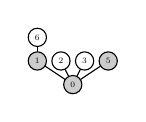
\begin{tikzpicture}[scale=.2]
          \node[circle, scale=0.4286, fill=white!80!black, draw=black] (tid0) at (3,1.5){\scriptsize{0}};
          \node[circle, scale=0.4286, fill=white!80!black, draw=black] (tid1) at (0.75,3){\scriptsize{1}};
          \node[circle, scale=0.4286, fill, task_scheduled] (tid6) at (0.75,4.5){\scriptsize{6}};
          \draw[](tid1) -- (tid6);
          \node[circle, scale=0.4286, fill, task_scheduled] (tid2) at (2.25,3){\scriptsize{2}};
          \node[circle, scale=0.4286, fill, task_scheduled] (tid3) at (3.75,3){\scriptsize{3}};
          \node[circle, scale=0.4286, fill=white!80!black, draw=black] (tid5) at (5.25,3){\scriptsize{5}};
          \draw[](tid0) -- (tid1);
          \draw[](tid0) -- (tid2);
          \draw[](tid0) -- (tid3);
          \draw[](tid0) -- (tid5);
        \end{tikzpicture}
      };
      & 
      \node[draw=black, rectangle split,  rectangle split parts=1] (sn0x9bd1828){
        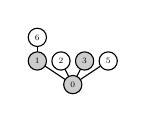
\begin{tikzpicture}[scale=.2]
          \node[circle, scale=0.4286, fill=white!80!black, draw=black] (tid0) at (3,1.5){\scriptsize{0}};
          \node[circle, scale=0.4286, fill=white!80!black, draw=black] (tid1) at (0.75,3){\scriptsize{1}};
          \node[circle, scale=0.4286, fill, task_scheduled] (tid6) at (0.75,4.5){\scriptsize{6}};
          \draw[](tid1) -- (tid6);
          \node[circle, scale=0.4286, fill, task_scheduled] (tid2) at (2.25,3){\scriptsize{2}};
          \node[circle, scale=0.4286, fill=white!80!black, draw=black] (tid3) at (3.75,3){\scriptsize{3}};
          \node[circle, scale=0.4286, fill, task_scheduled] (tid5) at (5.25,3){\scriptsize{5}};
          \draw[](tid0) -- (tid1);
          \draw[](tid0) -- (tid2);
          \draw[](tid0) -- (tid3);
          \draw[](tid0) -- (tid5);
        \end{tikzpicture}
      };
      & 
      \node[draw=black, rectangle split,  rectangle split parts=1] (sn0x9bd0f28){
        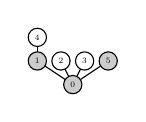
\begin{tikzpicture}[scale=.2]
          \node[circle, scale=0.4286, fill=white!80!black, draw=black] (tid0) at (3,1.5){\scriptsize{0}};
          \node[circle, scale=0.4286, fill=white!80!black, draw=black] (tid1) at (0.75,3){\scriptsize{1}};
          \node[circle, scale=0.4286, fill, task_scheduled] (tid4) at (0.75,4.5){\scriptsize{4}};
          \draw[](tid1) -- (tid4);
          \node[circle, scale=0.4286, fill, task_scheduled] (tid2) at (2.25,3){\scriptsize{2}};
          \node[circle, scale=0.4286, fill, task_scheduled] (tid3) at (3.75,3){\scriptsize{3}};
          \node[circle, scale=0.4286, fill=white!80!black, draw=black] (tid5) at (5.25,3){\scriptsize{5}};
          \draw[](tid0) -- (tid1);
          \draw[](tid0) -- (tid2);
          \draw[](tid0) -- (tid3);
          \draw[](tid0) -- (tid5);
        \end{tikzpicture}
      };
      & 
      \node[draw=black, rectangle split,  rectangle split parts=1] (sn0x9bd2140){
        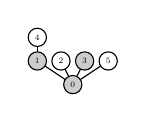
\begin{tikzpicture}[scale=.2]
          \node[circle, scale=0.4286, fill=white!80!black, draw=black] (tid0) at (3,1.5){\scriptsize{0}};
          \node[circle, scale=0.4286, fill=white!80!black, draw=black] (tid1) at (0.75,3){\scriptsize{1}};
          \node[circle, scale=0.4286, fill, task_scheduled] (tid4) at (0.75,4.5){\scriptsize{4}};
          \draw[](tid1) -- (tid4);
          \node[circle, scale=0.4286, fill, task_scheduled] (tid2) at (2.25,3){\scriptsize{2}};
          \node[circle, scale=0.4286, fill=white!80!black, draw=black] (tid3) at (3.75,3){\scriptsize{3}};
          \node[circle, scale=0.4286, fill, task_scheduled] (tid5) at (5.25,3){\scriptsize{5}};
          \draw[](tid0) -- (tid1);
          \draw[](tid0) -- (tid2);
          \draw[](tid0) -- (tid3);
          \draw[](tid0) -- (tid5);
        \end{tikzpicture}
      };
      & 
      \node[draw=black, rectangle split,  rectangle split parts=1] (sn0x9bc7440){
        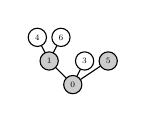
\begin{tikzpicture}[scale=.2]
          \node[circle, scale=0.4286, fill=white!80!black, draw=black] (tid0) at (3,1.5){\scriptsize{0}};
          \node[circle, scale=0.4286, fill=white!80!black, draw=black] (tid1) at (1.5,3){\scriptsize{1}};
          \node[circle, scale=0.4286, fill, task_scheduled] (tid4) at (0.75,4.5){\scriptsize{4}};
          \node[circle, scale=0.4286, fill, task_scheduled] (tid6) at (2.25,4.5){\scriptsize{6}};
          \draw[](tid1) -- (tid4);
          \draw[](tid1) -- (tid6);
          \node[circle, scale=0.4286, fill, task_scheduled] (tid3) at (3.75,3){\scriptsize{3}};
          \node[circle, scale=0.4286, fill=white!80!black, draw=black] (tid5) at (5.25,3){\scriptsize{5}};
          \draw[](tid0) -- (tid1);
          \draw[](tid0) -- (tid3);
          \draw[](tid0) -- (tid5);
        \end{tikzpicture}
      };
      & 
      \node[draw=black, rectangle split,  rectangle split parts=1] (sn0x9bd1530){
        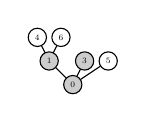
\begin{tikzpicture}[scale=.2]
          \node[circle, scale=0.4286, fill=white!80!black, draw=black] (tid0) at (3,1.5){\scriptsize{0}};
          \node[circle, scale=0.4286, fill=white!80!black, draw=black] (tid1) at (1.5,3){\scriptsize{1}};
          \node[circle, scale=0.4286, fill, task_scheduled] (tid4) at (0.75,4.5){\scriptsize{4}};
          \node[circle, scale=0.4286, fill, task_scheduled] (tid6) at (2.25,4.5){\scriptsize{6}};
          \draw[](tid1) -- (tid4);
          \draw[](tid1) -- (tid6);
          \node[circle, scale=0.4286, fill=white!80!black, draw=black] (tid3) at (3.75,3){\scriptsize{3}};
          \node[circle, scale=0.4286, fill, task_scheduled] (tid5) at (5.25,3){\scriptsize{5}};
          \draw[](tid0) -- (tid1);
          \draw[](tid0) -- (tid3);
          \draw[](tid0) -- (tid5);
        \end{tikzpicture}
      };
      & 
      \\
    };
  \end{scope}
  \draw (sn0x9bc9928.south) -- (sn0x9bc7440.north);
  \draw (sn0x9bc9928.south) -- (sn0x9bd1530.north);
  \draw (sn0x9bc9928.south) -- (sn0x9bcb370.north);
  \draw (sn0x9bc9928.south) -- (sn0x9bd1828.north);
  \draw (sn0x9bc9928.south) -- (sn0x9bd0f28.north);
  \draw (sn0x9bc9928.south) -- (sn0x9bd2140.north);
  \begin{scope}[yshift=-3cm]
    \draw[decorate,decoration={brace,mirror}] (-25.5,-17)
    --node[below, yshift=-.1cm]{Task 4 finished first} +(16.1,0);
    \draw[decorate,decoration={brace,mirror}] (-8.7,-17)
    --node[below, yshift=-.1cm]{Task 6 finished first} +(16.1,0);
    \draw[decorate,decoration={brace,mirror}] (8.2,-17)
    --node[below, yshift=-.1cm]{Task 2 finished first} +(16.1,0);
    % equivalences
    \draw[decorate,decoration={brace,mirror}] (-25.5,-22)
    --node[below, yshift=-.1cm]{4 equivalent snapshots} +(32.6,0);
    \draw[decorate,decoration={brace,mirror}] (8.2,-22)
    --node[below, yshift=-.1cm]{2 equivalent snapshots} +(16.1,0);
  \end{scope}
\end{tikzpicture}
